\section{Desarrollo}
\label{sec:desarrollo}

\subsection{Levantamiento de Requisitos}

\subsubsection{Técnicas Utilizadas}

% Entrevistas, revisión documental, etc.

\subsubsection{Actores del Sistema}

\begin{itemize}
    \item Vicedecano
    \item Director de Carrera
    \item Tutor
    \item Tribunal
    \item Estudiante
\end{itemize}

\subsubsection{Requisitos Funcionales}

\begin{itemize}
    \item \textbf{CU1 — Gestión de Usuarios:} Los usuarios del sistema (Vicedecano, Director, Tutor, Tribunal, Estudiante) pueden gestionar su perfil, subir su currículum en PDF y fotografía.
    \item \textbf{CU2 — Registro y Gestión de Manuscrito:} El Estudiante puede registrar su tesis o proyecto de grado en estado borrador, adjuntar archivos y enlazar repositorios (GitHub) o demos.
    \item \textbf{CU3 — Envío y Asignación para Revisión:} El Estudiante envía su manuscrito para revisión; el Director de Carrera designa un Tutor, quien puede aceptar o rechazar la asignación.
    \item \textbf{CU4 — Evaluación y Retroalimentación Académica:} El Tribunal evalúa el manuscrito asignando una puntuación y recomendación (aprobar, observar, rechazar); el Director también puede gestionar evaluaciones.
    \item \textbf{CU5 — Gestión Multicarrera y Configuración de Formatos:} El Admin gestiona las carreras, sus áreas de conocimiento y la configuración de formatos de presentación.
    \item \textbf{CU6 — Consulta Pública y Analítica:} El Público puede consultar las tesis publicadas, filtrar por carrera, categoría y palabras clave.
    \item \textbf{CU7 — Gestión de Pagos:} El Estudiante puede realizar pagos electrónicos (contado o crédito en 2 cuotas) mediante Stripe.
    \item \textbf{CU8 — Reportes y Estadísticas:} El Vicedecano, Director y Admin pueden generar reportes (tesis por carrera, por estado, por año, pagos, visitas, etc.) y exportarlos a CSV.
\end{itemize}

En la Figura~\ref{fig:casos-de-uso} se presenta el diagrama de casos de uso del sistema, donde se muestran los actores identificados y los casos de uso definidos.

\begin{figure}[H]
    \centering
    \caption{Diagrama de casos de uso del sistema.}
    \label{fig:casos-de-uso}
    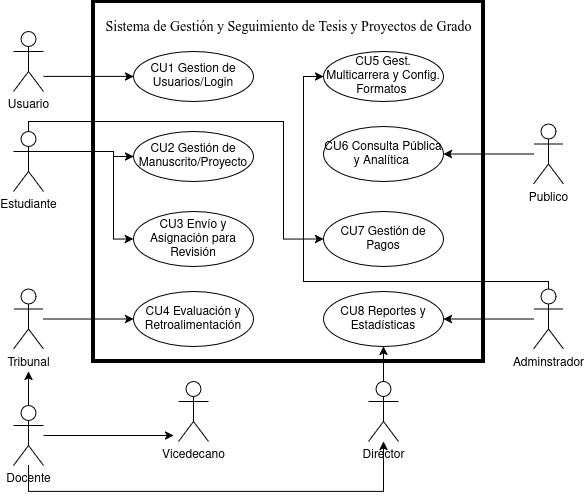
\includegraphics[width=\textwidth]{./cap7/img/casos-de-uso.png}
\end{figure}

\subsubsection{Especificación de Casos de Uso}

A continuación se presentan las tablas descriptivas de cada caso de uso identificado, detallando actores, propósito, resumen, flujo principal y excepciones.

\begin{table}[H]
\centering
\caption{CU1 — Gestión de Usuarios.}
\label{tab:cu1}
\begin{tabular}{lp{10cm}}
\toprule
\textbf{Atributo} & \textbf{Descripción} \\
\midrule
Caso de Uso & CU1 — Gestión de Usuarios \\
Actores & Vicedecano, Director, Tutor, Tribunal, Estudiante, Admin \\
Propósito & Permitir el registro, autenticación y gestión de perfiles de usuario del sistema, incluyendo la carga de currículum en PDF y fotografía. \\
Resumen & Los usuarios del sistema pueden registrarse, iniciar sesión y gestionar su perfil personal. Cada usuario tiene un rol asignado que determina los permisos dentro del sistema. El administrador puede gestionar todos los usuarios. \\
Flujo Principal & 1. El usuario accede al formulario de registro o inicio de sesión. \\
& 2. El sistema valida las credenciales ingresadas. \\
& 3. El usuario accede a su perfil y puede editar sus datos personales. \\
& 4. El usuario sube su fotografía y currículum en formato PDF. \\
& 5. El sistema guarda los cambios y muestra confirmación. \\
Excepciones & El correo electrónico ya está registrado. \\
& El formato de archivo no es válido (solo PDF para CV, JPG/PNG para foto). \\
& El tamaño del archivo supera el límite permitido. \\
\bottomrule
\end{tabular}
\end{table}

\begin{table}[H]
\centering
\caption{CU2 — Registro y Gestión de Manuscrito.}
\label{tab:cu2}
\begin{tabular}{lp{10cm}}
\toprule
\textbf{Atributo} & \textbf{Descripción} \\
\midrule
Caso de Uso & CU2 — Registro y Gestión de Manuscrito \\
Actores & Estudiante \\
Propósito & Permitir al estudiante registrar su tesis o proyecto de grado en estado borrador, adjuntar archivos y enlazar repositorios externos. \\
Resumen & El estudiante registra un nuevo manuscrito completando los datos requeridos (título, resumen, carrera, categoría). Puede adjuntar archivos PDF, enlazar un repositorio GitHub o una demo en línea. El manuscrito se guarda en estado borrador hasta que el estudiante decida enviarlo a revisión. \\
Flujo Principal & 1. El estudiante accede a la sección ``Mis Proyectos''. \\
& 2. Selecciona ``Nuevo Proyecto''. \\
& 3. Completa los campos del formulario (título, resumen, carrera, categoría). \\
& 4. Adjunta archivos PDF del manuscrito. \\
& 5. Opcionalmente, enlaza un repositorio GitHub o URL de demo. \\
& 6. Guarda el manuscrito en estado borrador. \\
& 7. El sistema muestra confirmación y el manuscrito queda visible en ``Mis Proyectos''. \\
Excepciones & El título ya existe en el sistema. \\
& El archivo adjunto excede el tamaño máximo permitido. \\
& El formato del archivo no es PDF. \\
& La URL del repositorio no es válida. \\
\bottomrule
\end{tabular}
\end{table}

\begin{table}[H]
\centering
\caption{CU3 — Envío y Asignación para Revisión.}
\label{tab:cu3}
\begin{tabular}{lp{10cm}}
\toprule
\textbf{Atributo} & \textbf{Descripción} \\
\midrule
Caso de Uso & CU3 — Envío y Asignación para Revisión \\
Actores & Estudiante, Director de Carrera, Tutor \\
Propósito & Gestionar el envío del manuscrito a revisión y la asignación de un tutor por parte del director de carrera. \\
Resumen & El estudiante envía su manuscrito en estado borrador para revisión. El director de carrera recibe una notificación y designa un tutor para el proyecto. El tutor asignado puede aceptar o rechazar la asignación. Si la rechaza, el director debe designar otro tutor. \\
Flujo Principal & 1. El estudiante envía su manuscrito para revisión desde ``Mis Proyectos''. \\
& 2. El sistema notifica al director de carrera. \\
& 3. El director accede al panel de administración y designa un tutor. \\
& 4. El sistema notifica al tutor asignado. \\
& 5. El tutor acepta la asignación. \\
& 6. El sistema actualiza el estado del manuscrito a ``en revisión''. \\
Excepciones & El tutor rechaza la asignación; el director debe designar otro tutor. \\
& El estudiante no ha completado los campos obligatorios del manuscrito. \\
& No hay tutores disponibles para la carrera del proyecto. \\
\bottomrule
\end{tabular}
\end{table}

\begin{table}[H]
\centering
\caption{CU4 — Evaluación y Retroalimentación Académica.}
\label{tab:cu4}
\begin{tabular}{lp{10cm}}
\toprule
\textbf{Atributo} & \textbf{Descripción} \\
\midrule
Caso de Uso & CU4 — Evaluación y Retroalimentación Académica \\
Actores & Tribunal, Director de Carrera \\
Propósito & Permitir al tribunal evaluar el manuscrito asignando una puntuación y una recomendación, y al director gestionar las evaluaciones. \\
Resumen & El tribunal accede a los manuscritos asignados, los revisa y emite una evaluación con puntuación numérica (1-100) y recomendación (aprobar, observar, rechazar). El director de carrera puede gestionar las evaluaciones y visualizar los resultados. \\
Flujo Principal & 1. El tribunal accede a la sección ``Mis Evaluaciones''. \\
& 2. Selecciona un manuscrito pendiente de evaluar. \\
& 3. Revisa el contenido del manuscrito y los archivos adjuntos. \\
& 4. Ingresa la puntuación (1--100) y selecciona una recomendación. \\
& 5. Agrega comentarios y retroalimentación. \\
& 6. Envía la evaluación. \\
& 7. El sistema registra la evaluación y notifica al director. \\
Excepciones & La puntuación está fuera del rango permitido (1--100). \\
& El tribunal intenta evaluar un manuscrito no asignado. \\
& El manuscrito ya fue evaluado por el mismo tribunal. \\
\bottomrule
\end{tabular}
\end{table}

\begin{table}[H]
\centering
\caption{CU5 — Gestión Multicarrera y Configuración de Formatos.}
\label{tab:cu5}
\begin{tabular}{lp{10cm}}
\toprule
\textbf{Atributo} & \textbf{Descripción} \\
\midrule
Caso de Uso & CU5 — Gestión Multicarrera y Configuración de Formatos \\
Actores & Admin \\
Propósito & Gestionar las carreras, áreas de conocimiento y la configuración de formatos de presentación del sistema. \\
Resumen & El administrador puede crear, editar y eliminar carreras universitarias, así como gestionar las áreas de conocimiento asociadas a cada carrera. También puede configurar los formatos de presentación (plantillas, requisitos) que aplicarán a los manuscritos de cada carrera. \\
Flujo Principal & 1. El admin accede al panel de administración. \\
& 2. Selecciona la opción ``Carreras''. \\
& 3. Crea una nueva carrera o edita una existente. \\
& 4. Asocia áreas de conocimiento a la carrera. \\
& 5. Configura los formatos de presentación requeridos. \\
& 6. Guarda los cambios. \\
& 7. El sistema actualiza la configuración. \\
Excepciones & El nombre de la carrera ya existe. \\
& Se intenta eliminar una carrera con manuscritos asociados. \\
& El formato de presentación contiene errores de validación. \\
\bottomrule
\end{tabular}
\end{table}

\begin{table}[H]
\centering
\caption{CU6 — Consulta Pública y Analítica.}
\label{tab:cu6}
\begin{tabular}{lp{10cm}}
\toprule
\textbf{Atributo} & \textbf{Descripción} \\
\midrule
Caso de Uso & CU6 — Consulta Pública y Analítica \\
Actores & Público \\
Propósito & Permitir la consulta de tesis publicadas con filtros por carrera, categoría y palabras clave. \\
Resumen & Cualquier persona sin autenticación puede acceder a la página pública del sistema, consultar las tesis que han sido publicadas, aplicar filtros de búsqueda y ver el detalle de cada tesis. \\
Flujo Principal & 1. El usuario accede a la página principal del sistema. \\
& 2. Visualiza la lista de tesis publicadas. \\
& 3. Aplica filtros por carrera, categoría o palabras clave. \\
& 4. El sistema actualiza los resultados según los filtros. \\
& 5. El usuario selecciona una tesis para ver su detalle. \\
& 6. El sistema muestra la información completa de la tesis. \\
Excepciones & No hay tesis publicadas que coincidan con los filtros aplicados. \\
& La tesis seleccionada fue retirada o despublicada. \\
\bottomrule
\end{tabular}
\end{table}

\begin{table}[H]
\centering
\caption{CU7 — Gestión de Pagos.}
\label{tab:cu7}
\begin{tabular}{lp{10cm}}
\toprule
\textbf{Atributo} & \textbf{Descripción} \\
\midrule
Caso de Uso & CU7 — Gestión de Pagos \\
Actores & Estudiante \\
Propósito & Permitir al estudiante realizar pagos electrónicos mediante Stripe, en modalidades de contado o crédito en 2 cuotas. \\
Resumen & El estudiante puede realizar el pago de su proyecto de grado a través de la plataforma Stripe. Puede elegir entre pago al contado o crédito en 2 cuotas. El sistema registra la transacción y actualiza el estado de pago del estudiante. \\
Flujo Principal & 1. El estudiante accede a la sección ``Pagos''. \\
& 2. Selecciona la modalidad de pago (contado o crédito 2 cuotas). \\
& 3. Ingresa los datos de su tarjeta en el formulario de Stripe. \\
& 4. Stripe procesa el pago. \\
& 5. El sistema registra la transacción exitosa. \\
& 6. El sistema actualiza el estado de pago del estudiante. \\
& 7. Se muestra comprobante de pago. \\
Excepciones & El pago es rechazado por Stripe (fondos insuficientes, tarjeta inválida). \\
& La conexión con Stripe falla durante el proceso. \\
& El estudiante ya tiene un pago registrado para el período. \\
\bottomrule
\end{tabular}
\end{table}

\begin{table}[H]
\centering
\caption{CU8 — Reportes y Estadísticas.}
\label{tab:cu8}
\begin{tabular}{lp{10cm}}
\toprule
\textbf{Atributo} & \textbf{Descripción} \\
\midrule
Caso de Uso & CU8 — Reportes y Estadísticas \\
Actores & Vicedecano, Director de Carrera, Admin \\
Propósito & Generar reportes y estadísticas del sistema con opción de exportación a CSV. \\
Resumen & Los usuarios con permisos de gestión pueden generar reportes sobre tesis (por carrera, estado, año), pagos realizados, visitas a tesis, entre otros. Los reportes pueden visualizarse en pantalla y exportarse a formato CSV para su procesamiento externo. \\
Flujo Principal & 1. El usuario accede a la sección ``Reportes''. \\
& 2. Selecciona el tipo de reporte a generar. \\
& 3. Aplica filtros (carrera, estado, rango de fechas). \\
& 4. El sistema genera el reporte con los datos solicitados. \\
& 5. El usuario visualiza los resultados en pantalla. \\
& 6. El usuario selecciona exportar a CSV. \\
& 7. El sistema descarga el archivo CSV. \\
Excepciones & No hay datos disponibles para los filtros seleccionados. \\
& El rango de fechas es inválido (fecha final menor a fecha inicial). \\
& El usuario no tiene permisos para acceder al reporte solicitado. \\
\bottomrule
\end{tabular}
\end{table}

% ------------------------------------------------------------------
\subsection{Modelado con UWE}

\subsubsection{Modelo de Contenido}

El modelo de contenido define la estructura de la información del sistema mediante un diagrama de clases UML. En la Figura~\ref{fig:diagrama-clases} se presentan las entidades principales del sistema con sus atributos y relaciones.

\begin{figure}[H]
    \centering
    \caption{Diagrama de clases del sistema.}
    \label{fig:diagrama-clases}
    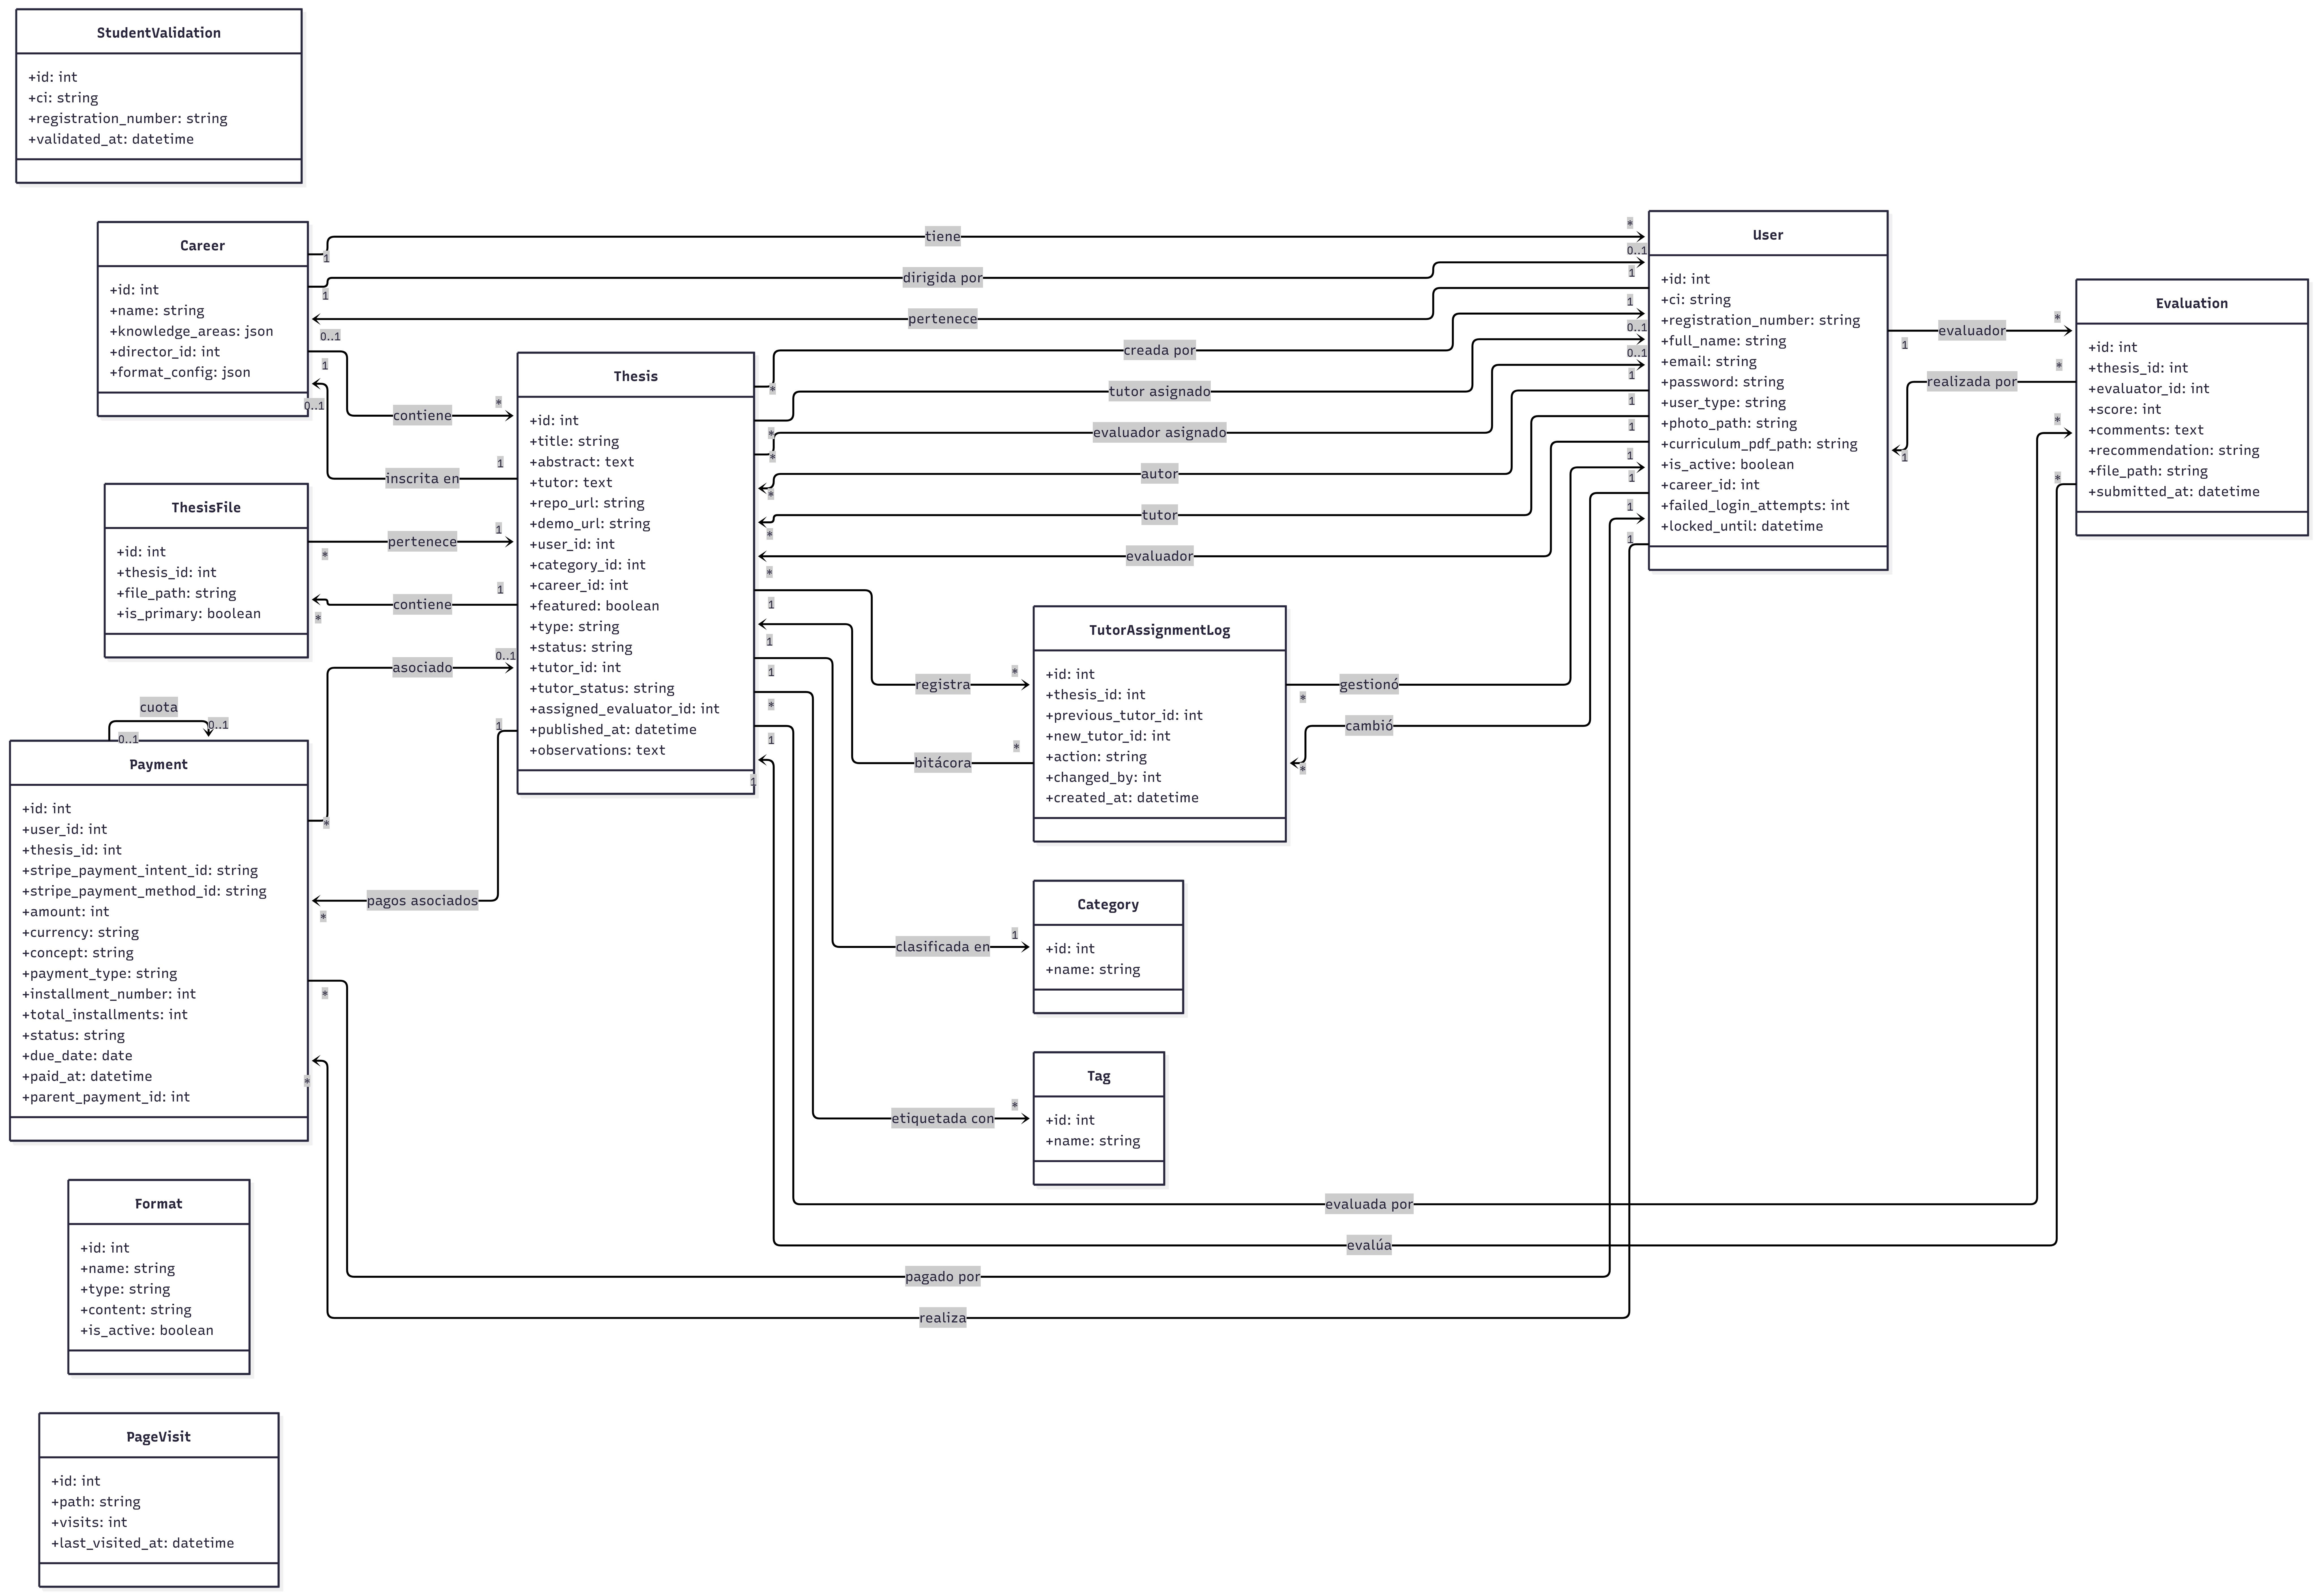
\includegraphics[width=\textwidth]{./cap7/img/clases.png}
\end{figure}

\subsubsection{Modelo de Navegación}

El modelo de navegación define las rutas de acceso a la información según el perfil del usuario. A continuación se presentan los diagramas organizados por grupos de roles.

\begin{figure}[H]
    \centering
    \caption{Diagrama de navegación del sistema por perfil.}
    \label{fig:navegacion}
    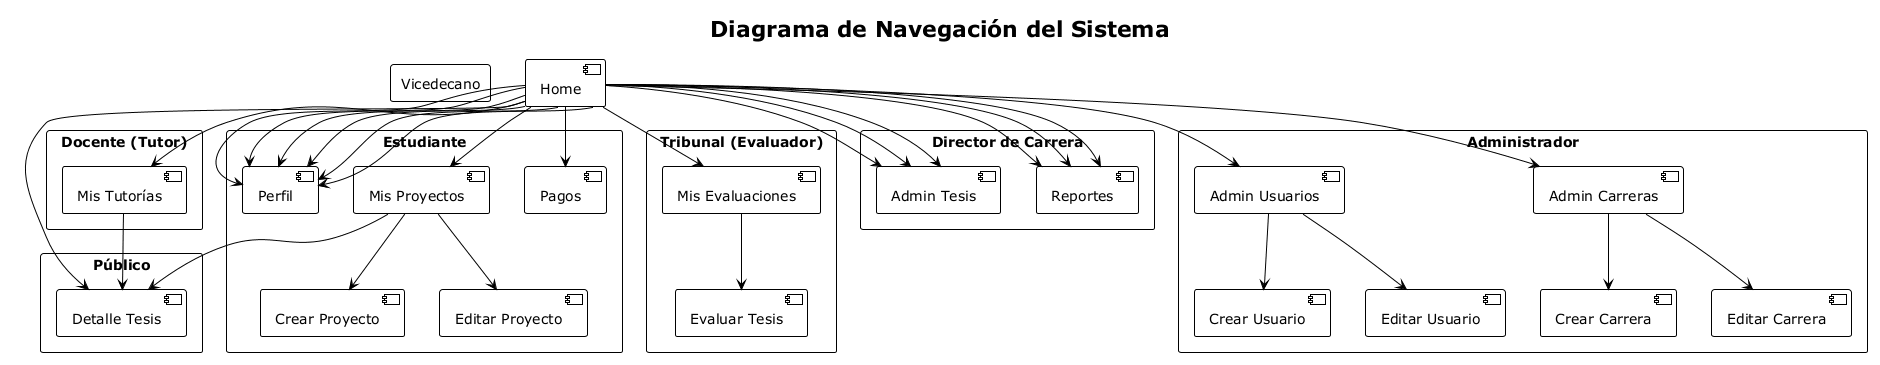
\includegraphics[width=\textwidth]{./cap7/img/navegacion.png}
\end{figure}

\subsubsection{Modelo de Presentación}

% Wireframes o prototipos

\subsubsection{Modelo de Procesos}

% Diagramas de actividad por flujo

% ------------------------------------------------------------------
\subsection{Modelo de Datos}

% Diagrama entidad-relación, principales tablas

% ------------------------------------------------------------------
\subsection{Arquitectura del Sistema}

El sistema sigue una arquitectura monolítica basada en Laravel con Inertia.js, combinando los patrones MVC (Model-View-Controller) del lado del servidor y MVVM (Model-View-ViewModel) del lado del cliente.

\begin{figure}[H]
    \centering
    \caption{Diagrama de arquitectura del sistema.}
    \label{fig:arquitectura}
    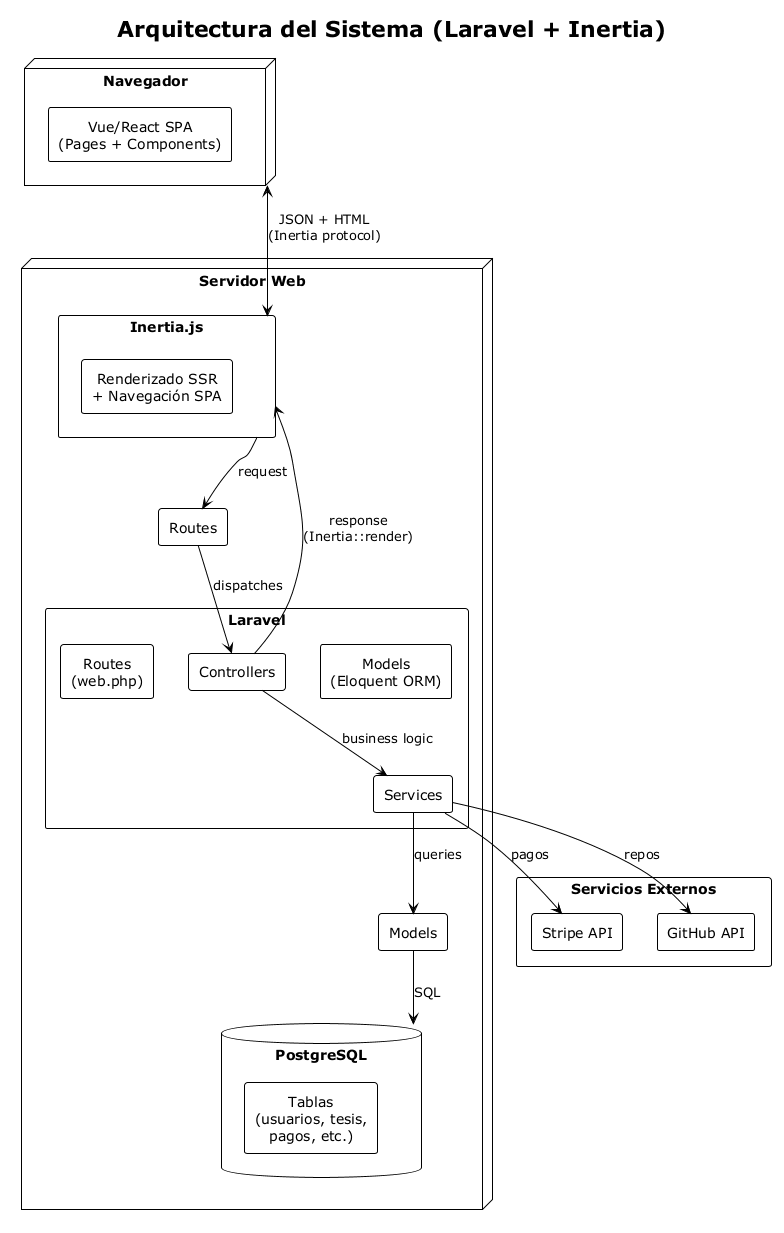
\includegraphics[width=\textwidth]{./cap7/img/arquitectura.png}
\end{figure}

\subsubsection{Capa de Presentación (Cliente)}

El frontend se implementa con Vue.js (o React) como SPA, gestionado por Inertia.js. Este enfoque evita la construcción de una API REST tradicional: Inertia actúa como un puente que permite renderizar componentes desde el servidor manteniendo la experiencia de navegación SPA en el cliente. El estado y la lógica de presentación se manejan con el patrón MVVM, donde los componentes Vue son la Vista y las props recibidas del controlador Laravel actúan como el ViewModel.

\subsubsection{Capa de Aplicación (Servidor)}

Laravel implementa el patrón MVC clásico:

\begin{itemize}
    \item \textbf{Routes:} Definidas en \texttt{web.php}, manejan las peticiones HTTP y las dirigen a los controladores correspondientes, con middleware de autenticación y roles.
    \item \textbf{Controllers:} Procesan las peticiones, validan datos y retornan respuestas Inertia o redirecciones. Cada caso de uso (CU1--CU8) tiene su propio controlador o grupo de controladores.
    \item \textbf{Services:} Encapsulan la lógica de negocio (cálculo de pagos, generación de reportes, asignación de tutores), manteniendo los controladores ligeros.
    \item \textbf{Models:} Representan las entidades del sistema (User, Thesis, Payment, Evaluation, etc.) mediante Eloquent ORM, gestionando la interacción con la base de datos.
\end{itemize}

\subsubsection*{Capa de Datos}

La base de datos PostgreSQL almacena toda la información del sistema: usuarios, tesis, archivos adjuntos, evaluaciones, pagos, carreras y configuraciones. Las migraciones de Laravel gestionan el esquema y las relaciones entre tablas.

\subsubsection*{Servicios Externos}

\begin{itemize}
    \item \textbf{Stripe:} Procesamiento de pagos electrónicos en las modalidades de contado y crédito en 2 cuotas.
    \item \textbf{GitHub API:} Verificación y enlace de repositorios de código fuente desde los manuscritos de tesis.
\end{itemize}

% ------------------------------------------------------------------
\subsection{Desarrollo por Sprints}

El desarrollo del sistema se organizó en 8 sprints de una semana de duración cada uno, desde el 22 de mayo hasta el 4 de julio de 2026. Cada sprint abordó uno de los casos de uso definidos, desglosado en historias de usuario (HU) con su estimación de esfuerzo en horas, prioridad y estado.

\subsubsection{Historias de Usuario}

En la Tabla~\ref{tab:hu} se presentan las 20 historias de usuario definidas para el sistema, con su prioridad, esfuerzo estimado, sprint asignado y caso de uso relacionado.

\medskip
\noindent
\begin{table}[H]
\centering
\caption{Historias de usuario del sistema.}
\label{tab:hu}
\begin{tabular}{lccccc}
\toprule
\textbf{HU} & \textbf{Título} & \textbf{Prioridad} & \textbf{Esfuerzo (h)} & \textbf{Sprint} & \textbf{CU} \\
\midrule
HU-01 & Registro de usuarios & Alta & 8 & 1 & CU1 \\
HU-02 & Inicio de sesión & Alta & 6 & 1 & CU1 \\
HU-03 & Gestión de perfil (CV y foto) & Media & 6 & 1 & CU1 \\
HU-04 & Recuperación de contraseña & Media & 4 & 1 & CU1 \\
HU-05 & Registrar tesis/proyecto en borrador & Alta & 8 & 2 & CU2 \\
HU-06 & Adjuntar archivos al manuscrito & Alta & 6 & 2 & CU2 \\
HU-07 & Enlazar repositorio GitHub/Demo & Media & 4 & 2 & CU2 \\
HU-08 & Enviar manuscrito a revisión & Alta & 6 & 3 & CU3 \\
HU-09 & Designar tutor por el director & Alta & 4 & 3 & CU3 \\
HU-10 & Aceptar/rechazar asignación (tutor) & Alta & 4 & 3 & CU3 \\
HU-11 & Evaluar manuscrito con puntuación & Alta & 8 & 4 & CU4 \\
HU-12 & Retroalimentación y recomendación & Alta & 6 & 4 & CU4 \\
HU-13 & Gestionar carreras y áreas & Alta & 8 & 5 & CU5 \\
HU-14 & Configurar formatos por carrera & Media & 6 & 5 & CU5 \\
HU-15 & Consultar tesis publicadas (público) & Alta & 6 & 6 & CU6 \\
HU-16 & Filtrar por carrera, categoría y palabras clave & Media & 4 & 6 & CU6 \\
HU-17 & Realizar pago en línea (contado) & Alta & 6 & 7 & CU7 \\
HU-18 & Realizar pago en línea (crédito 2 cuotas) & Alta & 8 & 7 & CU7 \\
HU-19 & Generar reportes de tesis, pagos y visitas & Alta & 6 & 8 & CU8 \\
HU-20 & Exportar reportes a CSV & Media & 4 & 8 & CU8 \\
\bottomrule
\end{tabular}
\end{table}
\medskip

\subsubsection{Sprint 1: Gestión de Usuarios}
\label{sprint:1}

\textbf{Duración:} 22 de mayo – 27 de mayo de 2026 (6 días). \\
\textbf{Objetivo:} Implementar el registro, autenticación y gestión de perfiles de usuarios del sistema, incluyendo la carga de CV y fotografía.

\begin{center}
\begin{tabular}{lcccc}
\toprule
\textbf{HU} & \textbf{Título} & \textbf{Esfuerzo (h)} & \textbf{Prioridad} & \textbf{Estado} \\
\midrule
HU-01 & Registro de usuarios & 8 & Alta & Completado \\
HU-02 & Inicio de sesión & 6 & Alta & Completado \\
HU-03 & Gestión de perfil (CV y foto) & 6 & Media & Completado \\
HU-04 & Recuperación de contraseña & 4 & Media & Completado \\
\bottomrule
\end{tabular}
\end{center}

\textbf{Entregable:} Módulo de autenticación y perfiles de usuario funcional, con roles definidos (Vicedecano, Director, Tutor, Tribunal, Estudiante, Admin).

\subsubsection{Sprint 2: Registro y Gestión de Manuscritos}
\label{sprint:2}

\textbf{Duración:} 28 de mayo – 2 de junio de 2026 (6 días). \\
\textbf{Objetivo:} Permitir al estudiante registrar su tesis o proyecto en estado borrador, adjuntar archivos y enlazar repositorios externos.

\begin{center}
\begin{tabular}{lcccc}
\toprule
\textbf{HU} & \textbf{Título} & \textbf{Esfuerzo (h)} & \textbf{Prioridad} & \textbf{Estado} \\
\midrule
HU-05 & Registrar tesis/proyecto en borrador & 8 & Alta & Completado \\
HU-06 & Adjuntar archivos al manuscrito & 6 & Alta & Completado \\
HU-07 & Enlazar repositorio GitHub/Demo & 4 & Media & Completado \\
\bottomrule
\end{tabular}
\end{center}

\textbf{Entregable:} Formulario de registro de tesis con subida de archivos y enlace a repositorio externo.

\subsubsection{Sprint 3: Asignación de Tutores y Tribunales}
\label{sprint:3}

\textbf{Duración:} 3 de junio – 8 de junio de 2026 (6 días). \\
\textbf{Objetivo:} Implementar el flujo de envío de manuscrito a revisión y la asignación de tutores por el director de carrera.

\begin{center}
\begin{tabular}{lcccc}
\toprule
\textbf{HU} & \textbf{Título} & \textbf{Esfuerzo (h)} & \textbf{Prioridad} & \textbf{Estado} \\
\midrule
HU-08 & Enviar manuscrito a revisión & 6 & Alta & Completado \\
HU-09 & Designar tutor por el director & 4 & Alta & Completado \\
HU-10 & Aceptar/rechazar asignación (tutor) & 4 & Alta & Completado \\
\bottomrule
\end{tabular}
\end{center}

\textbf{Entregable:} Flujo de asignación de tutores con notificaciones y aceptación/rechazo.

\subsubsection{Sprint 4: Evaluación y Retroalimentación}
\label{sprint:4}

\textbf{Duración:} 9 de junio – 14 de junio de 2026 (6 días). \\
\textbf{Objetivo:} Desarrollar el módulo de evaluación de manuscritos por parte del tribunal, incluyendo puntuación y recomendación.

\begin{center}
\begin{tabular}{lcccc}
\toprule
\textbf{HU} & \textbf{Título} & \textbf{Esfuerzo (h)} & \textbf{Prioridad} & \textbf{Estado} \\
\midrule
HU-11 & Evaluar manuscrito con puntuación & 8 & Alta & Completado \\
HU-12 & Retroalimentación y recomendación & 6 & Alta & Completado \\
\bottomrule
\end{tabular}
\end{center}

\textbf{Entregable:} Módulo de evaluación con puntuación (1--100), recomendación (aprobar/observar/rechazar) y comentarios.

\subsubsection{Sprint 5: Gestión Multicarrera y Configuración de Formatos}
\label{sprint:5}

\textbf{Duración:} 15 de junio – 20 de junio de 2026 (6 días). \\
\textbf{Objetivo:} Implementar la gestión de carreras, áreas de conocimiento y configuración de formatos de presentación.

\begin{center}
\begin{tabular}{lcccc}
\toprule
\textbf{HU} & \textbf{Título} & \textbf{Esfuerzo (h)} & \textbf{Prioridad} & \textbf{Estado} \\
\midrule
HU-13 & Gestionar carreras y áreas & 8 & Alta & Completado \\
HU-14 & Configurar formatos por carrera & 6 & Media & Completado \\
\bottomrule
\end{tabular}
\end{center}

\textbf{Entregable:} Panel de administración de carreras con CRUD completo y configuración de formatos.

\subsubsection{Sprint 6: Consulta Pública y Analítica}
\label{sprint:6}

\textbf{Duración:} 21 de junio – 26 de junio de 2026 (6 días). \\
\textbf{Objetivo:} Desarrollar la consulta pública de tesis publicadas con filtros por carrera, categoría y palabras clave.

\begin{center}
\begin{tabular}{lcccc}
\toprule
\textbf{HU} & \textbf{Título} & \textbf{Esfuerzo (h)} & \textbf{Prioridad} & \textbf{Estado} \\
\midrule
HU-15 & Consultar tesis publicadas (público) & 6 & Alta & Completado \\
HU-16 & Filtrar por carrera, categoría y palabras clave & 4 & Media & Completado \\
\bottomrule
\end{tabular}
\end{center}

\textbf{Entregable:} Página pública de consulta de tesis con buscador y filtros.

\subsubsection{Sprint 7: Gestión de Pagos}
\label{sprint:7}

\textbf{Duración:} 27 de junio – 2 de julio de 2026 (6 días). \\
\textbf{Objetivo:} Integrar pagos electrónicos mediante Stripe, ofreciendo opciones de contado y crédito en 2 cuotas.

\begin{center}
\begin{tabular}{lcccc}
\toprule
\textbf{HU} & \textbf{Título} & \textbf{Esfuerzo (h)} & \textbf{Prioridad} & \textbf{Estado} \\
\midrule
HU-17 & Realizar pago en línea (contado) & 6 & Alta & Completado \\
HU-18 & Realizar pago en línea (crédito 2 cuotas) & 8 & Alta & Completado \\
\bottomrule
\end{tabular}
\end{center}

\textbf{Entregable:} Módulo de pagos integrado con Stripe, persistencia de transacciones y registro de deuda para modalidad crédito.

\subsubsection{Sprint 8: Reportes y Estadísticas}
\label{sprint:8}

\textbf{Duración:} 3 de julio – 4 de julio de 2026 (2 días). \\
\textbf{Objetivo:} Implementar la generación de reportes y estadísticas del sistema con exportación a CSV.

\begin{center}
\begin{tabular}{lcccc}
\toprule
\textbf{HU} & \textbf{Título} & \textbf{Esfuerzo (h)} & \textbf{Prioridad} & \textbf{Estado} \\
\midrule
HU-19 & Generar reportes de tesis, pagos y visitas & 6 & Alta & Completado \\
HU-20 & Exportar reportes a CSV & 4 & Media & Completado \\
\bottomrule
\end{tabular}
\end{center}

\textbf{Entregable:} Módulo de reportes con filtros por carrera, estado, año y tipo, y exportación a CSV.

\subsubsection{Resumen de Esfuerzo}

En la Tabla~\ref{tab:resumen-esfuerzo} se presenta el resumen del esfuerzo total invertido por sprint.

\medskip
\noindent
\begin{table}[H]
\centering
\caption{Resumen de esfuerzo por sprint.}
\label{tab:resumen-esfuerzo}
\begin{tabular}{lccc}
\toprule
\textbf{Sprint} & \textbf{Caso de Uso} & \textbf{Duración} & \textbf{Esfuerzo (h)} \\
\midrule
1 & CU1 -- Gestión de Usuarios & 22 may -- 27 may & 24 \\
2 & CU2 -- Registro y Gestión de Manuscritos & 28 may -- 2 jun & 18 \\
3 & CU3 -- Asignación de Tutores y Tribunales & 3 jun -- 8 jun & 14 \\
4 & CU4 -- Evaluación y Retroalimentación & 9 jun -- 14 jun & 14 \\
5 & CU5 -- Gestión Multicarrera y Configuración & 15 jun -- 20 jun & 14 \\
6 & CU6 -- Consulta Pública y Analítica & 21 jun -- 26 jun & 10 \\
7 & CU7 -- Gestión de Pagos & 27 jun -- 2 jul & 14 \\
8 & CU8 -- Reportes y Estadísticas & 3 jul -- 4 jul & 10 \\
\midrule
\multicolumn{3}{l}{\textbf{Total}} & \textbf{118 h} \\
\bottomrule
\end{tabular}
\end{table}
\medskip

% ------------------------------------------------------------------
\subsection{Interfaces del Sistema}

% Capturas de pantalla por módulo

\endinput
